\documentclass[../main.tex]{subfiles}
% !TeX root = ../main.tex
\begin{document}
	\section{Income and Equity}
	
	\subsection{Corporations}
	
	The corporate form of organization has several advantages. The major 
	advantage is the ease of raising large amounts of money because both large 
	and small investors can participate in corporate ownership. It is simple to 
	become an owner of corporate shares of stock and just as simple to sell 
	these shares in organized exchanges such as the New York Stock Exchange 
	(NYSE), Singapore Stock Exchange etc. These exchanges maintain markets in 
	which shares are bought and sold each business day. 
	
	Corporations are entities created by law that exists separately from their 
	owners and that have rights and privileges. As separate entities, 
	corporations can:
	\begin{itemize}[noitemsep]
		\item Own assets
		\item Incur liabilities
		\item Sue and be sued.
		\item Enter into contracts. Shareholders are not agents of the 
		corporation and cannot enter into contracts on the corporation's 
		behalf. 
	\end{itemize}
	Shareholder losses are also limited in the amounts invested in the 
	corporation and corporate creditors cannot make claims on the personal 
	assets of shareholders to satisfy corporate debt.
	
	The corporate  form of organization has several advantages:
	\begin{itemize}[noitemsep]
		\item It is a separate legal entity that can enter into contracts and 
		sue or be sued. 
		\item Shareholder losses are limited to the amount invested in the 
		corporation.
		\item Ownership rights are transferable. 
		\item The corporation continues in existence even when ownership 
		changes. 
		\item Shareholders are not agents of the corporation and cannot enter 
		into contracts on the corporation's behalf. 
		\item Capital needs can be made by selling more ownership in the 
		corporation. 
	\end{itemize}
	The disadvantages include:
	\begin{itemize}[noitemsep]
		\item Extra governmental regulations imposed on corporations and 
		corporate taxation of earnings. Corporations pay taxes on their 
		earnings and if they distribute a dividend to shareholders, the 
		shareholders pay taxes on the dividends earned. 
	\end{itemize}

	\subsubsection{Corporate Organization and Management}
	
	The ultimate control of a corporation rests with shareholders who  control 
	a corporation by electing its board of directors, or simply, directors. 
	
	\subsubsection{Corporate Ownership}
	
	Stockholders have several benefits:
	\begin{itemize}[noitemsep]
		\item Voting rights
		\item Dividends - Right to receive dividends when declared by the board 
		of directors
		\item Residual claims - In the event of liquidation, shareholders 
		share, according to their percentage ownership, in any remaining assets 
		after creditors are paid
		\item Preemptive rights - Existing shareholders may be given the first 
		chance to buy newly issued shares of stock before it is offered to 
		others.
	\end{itemize}
	
	\subsection{Equity vs Debt Financing}
	
	Equity financing has some advantages when compared to debt financing. 
	\begin{itemize}[noitemsep]
		\item Equity financing does not have to be repaid as does debt.
		\item Cash dividends to shareholders are optional, whereas interest 
		payments on debt are mandatory.
	\end{itemize}
	
	However, debt financing also has some advantages. 
	\begin{itemize}[noitemsep]
		\item Interest payments to creditors are tax deductible, but dividend 
		payments to shareholders are not.
		\item Selling additional shares of stock can dilute the ownership 
		percentage of current shareholders, but additional debt does not change 
		shareholder control. 
	\end{itemize}

	\subsubsection{Authorization, Issuance and Repurchase of Shares}
	
	There are several terms related to shares that we need to understand. 
	\textbf{Authorized shares} are the maximum number of shares of stock that 
	can be issued to the public. Authorized shares can be classified as either 
	issued or unissued. 
	\begin{itemize}[noitemsep]
	\item \textbf{Issued shares} are authorized shares of stock 
	that have been distributed to shareholders. Issued shares can be classified 
	as either outstanding shares or treasury shares. 
	\begin{itemize}[noitemsep]
		\item \textbf{Outstanding shares} are shares that are currently owned 
		by shareholders.  
		\item \textbf{Treasury shares} are shares that were once owned by 
		shareholders but the corporation repurchased the shares in the stock 
		market. Now, the corporation is the owner of those shares.
	\end{itemize}
	\item \textbf{Unissued shares} are authorized shares of stock that have 
	never been issued to shareholders.
	\end{itemize}

	\subsection{Basics of Share Capital}
	
	Corporations must disclose information related to their shares, such as par 
	value and number of shares authorized and issued.  We can also find the 
	number of shares actually issued by the company. Low par values are normal 
	in business.
	
	\begin{figure}[ht]
		\centering
		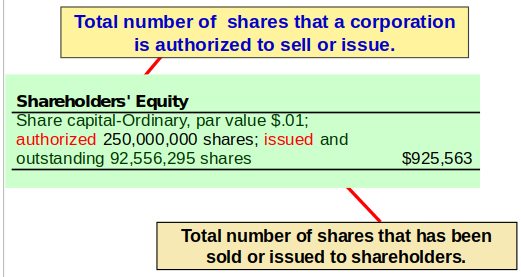
\includegraphics[width=\columnwidth]{images/c9/basics_share.png}
	\end{figure}
	
	\textbf{Par value} is an arbitrary amount assigned to each share.  Par 
	value is typically a nominal amount, and is not related in any manner to 
	market value which is the selling price of a share. In addition to par 
	value shares, some countries permit no-par, or stated value ordinary shares
	
	\subsubsection{Stock Exchanged between Investors}
	
	Once shares of stock are owned by the public, they may be bought and sold 
	in the open market. Such transactions do not involve the company or its 
	accounting records. The millions of shares that are bought and sold on the 
	New York Stock exchange each business day are examples of this type of 
	transaction.
	
	\subsubsection{Shares Issuance}
	
	At the \textbf{initial public offering (IPO)}, shares of stock are issued 
	to the public for the first time.
	
	At a later date, the company may wish to raise additional capital with 
	another issue of shares to the public. This is referred to as a 
	\textbf{seasoned new issue}. 
	
	\paragraph{Shares Issued at Par.} When par value shares are issued at par, 
	the Share Capital account is credited for the full amount.  
	
	\begin{figure}[ht]
		\centering
		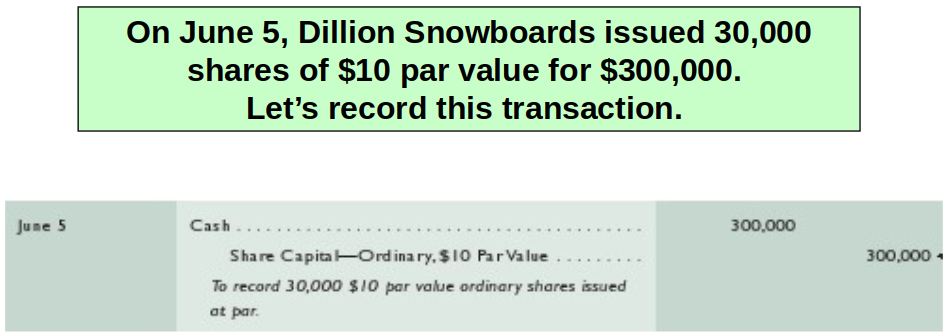
\includegraphics[width=\columnwidth]{images/c9/share_issue_par.png}
	\end{figure}
	
	\begin{figure}[ht]
		\centering
		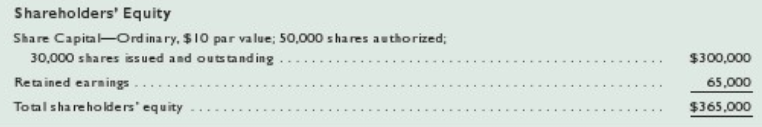
\includegraphics[width=\columnwidth]{images/c9/share_issue_par_eg1.png}
		\caption{Recording Shares Issued at Par}
	\end{figure}
	
	\paragraph{Shares Issued at Premium.} When par value shares are issued 
	above par, the Share Capital account is credited for the par value of the 
	shares sold. Remember that par value and market value are not related.  
	The difference between the par value of the shares and the market value of 
	the shares is credited to Share Premium.  If you added together the amount 
	of par value in the Share Capital account and the amount in the Share 
	Premium, you would have the market value of the issuance of the shares.  
	
	\begin{figure}[ht]
		\centering
		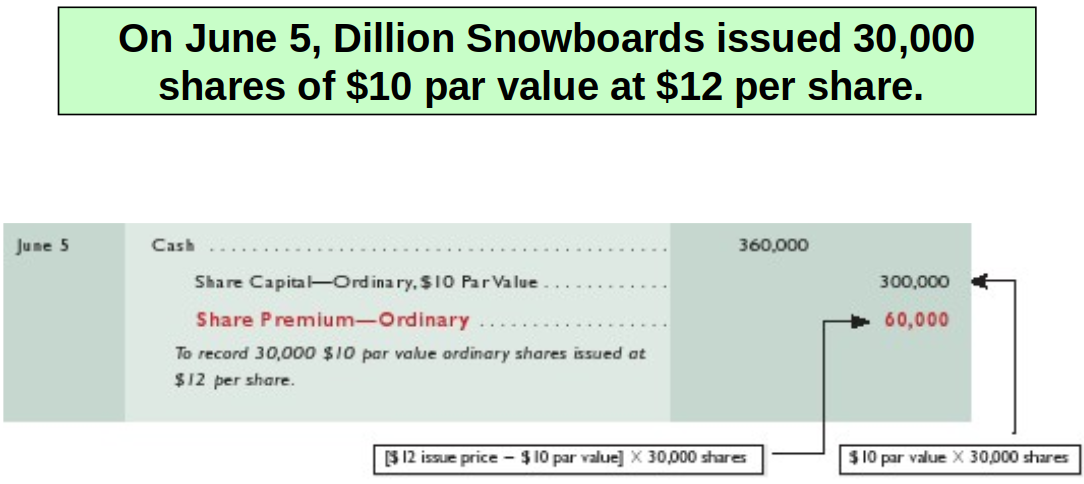
\includegraphics[width=\columnwidth]{images/c9/above_par_share_eg.png}
		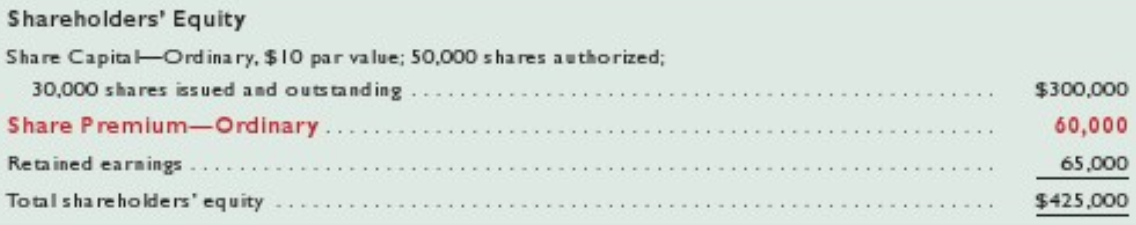
\includegraphics[width=\columnwidth]{images/c9/share_above_par_eg2.png}
		\caption{Recording Shares Issued Above Par}
	\end{figure}
	
	\paragraph{Issuing No-Par Value Shares.} When no-par value shares are 
	issued, the Share Capital account is credited for the amount of cash.

	\begin{figure}[ht]
		\centering
		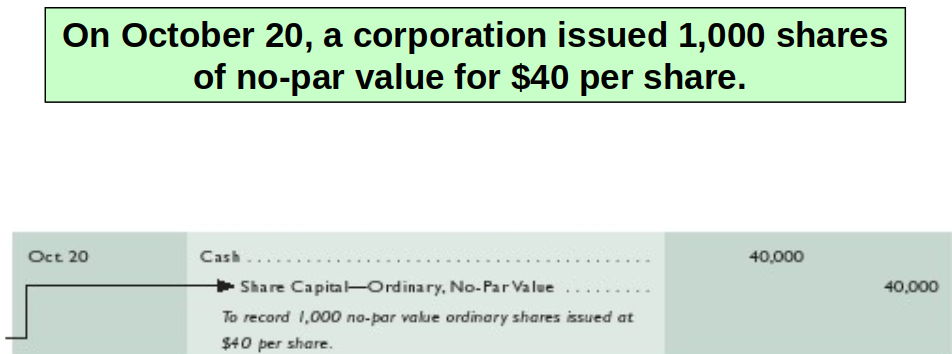
\includegraphics[width=\columnwidth]{images/c9/issuing_no_par_eg.png}
		\caption{Issuing at no-par}
	\end{figure}
	
	\paragraph{Issuing Stated Value Shares.} When stated value shares are 
	issued, the Share Capital account is credited for the stated value.  
	Remember that stated value and market value are not related.  The 
	difference between the stated value of the shares and the market value of 
	the shares is credited to Share Premium. If you added together the amount 
	of stated value in the Share Capital account and the amount in the Share 
	Premium, you would have the market value of the issuance of the shares. 
	
	\begin{figure}[ht!]
		\centering
		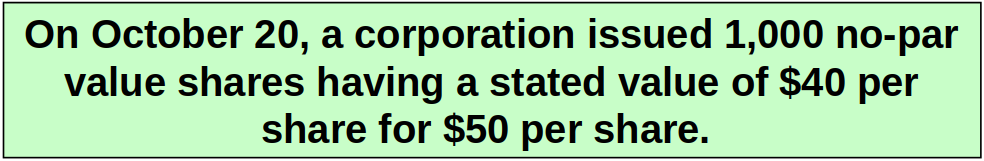
\includegraphics[width=\columnwidth]{images/c9/stated_eg1.png}
		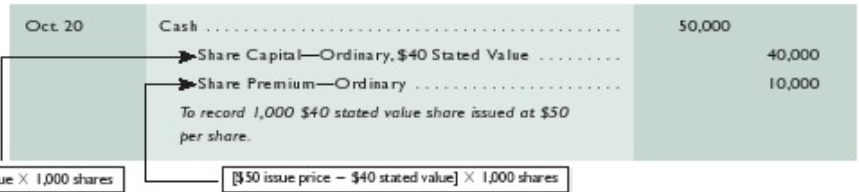
\includegraphics[width=\columnwidth]{images/c9/stated_eg2.png}
		\caption{Issuing Stated Value Shares}
	\end{figure}
	
	\paragraph{Issuing Shares for Noncash Assets.} The Share Capital account is 
	credited for the par value of the shares issued. The difference between the 
	par value of the shares and the market value of the assets received is 
	credited to Share Premium.  If you added together the amount of par value 
	in the Share Capital account and the amount in the Share Premium, you would 
	have the market value of the assets received.
	\begin{figure}[ht!]
		\centering
		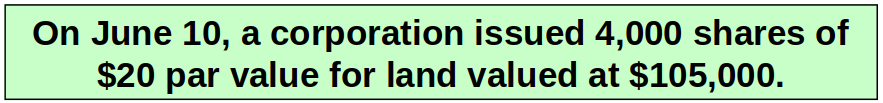
\includegraphics[width=\columnwidth]{images/c9/noncash_eg1.png}
		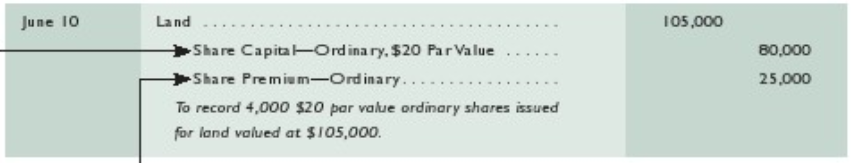
\includegraphics[width=\columnwidth]{images/c9/noncash_eg2.png}
		\caption{Issuing Stated Value Shares}
	\end{figure}
	
	\subsubsection{Cash Dividends}
	
	Shareholders receive a return on their investment in two ways: one is 
	through increases in the market value of the shares and one is through cash 
	dividends. To pay a cash dividend, a corporation must have two things:
	\begin{itemize}[noitemsep]
		\item Sufficient retained earnings to absorb the dividend without 
		creating a deficit; and
		\item Enough cash to pay the dividend.
	\end{itemize}
	
	There are three important dates to remember when discussing dividends:
	\begin{itemize}[noitemsep]
		\item The \textbf{date of declaration} is the date the directors 
		declare the dividend. At this time, a liability is created and must be 
		recorded.
		\begin{figure}[ht]
			\centering
			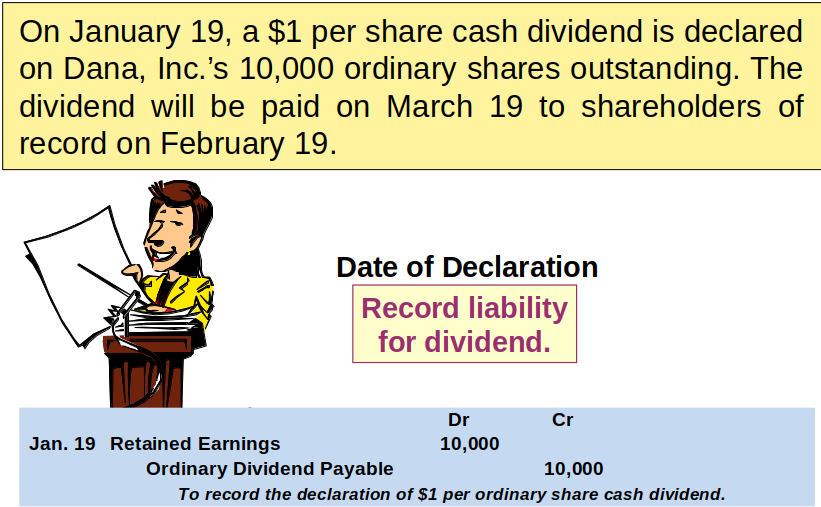
\includegraphics[width=\columnwidth]{images/c9/dividend_declaration.png}
			\caption{An alternative entry is to debit Dividends instead of 
			Retained Earnings. The balance in Dividends is then closed to 
			Retained Earnings at the end of the reporting period. The effect is 
			the same: Retained Earnings is decreased and a Dividend Payable is 
			increased}
		\end{figure}
		\item The \textbf{date of record} is important because you must own the 
		shares on this date to receive the dividend.  No entry is required in 
		the accounting records.  
		\item The \textbf{date of payment} is the date the corporation pays the 
		dividend to the shareholders who owned the shares on the record date.
				\begin{figure}[ht]
			\centering
			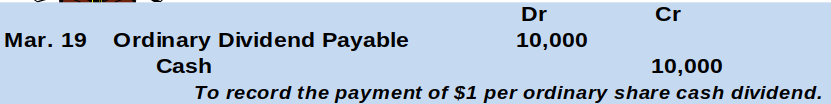
\includegraphics[width=\columnwidth]{images/c9/incoporated_date.png}
			\caption{Date of Payment}
		\end{figure}
	\end{itemize}
	
	\subsubsection{Bonus Issues or Share Dividends}
	
	Sometimes corporations will distribute additional shares as dividends.  
	Reasons for doing this include:
	\begin{itemize}[noitemsep]
		\item Keeping the market price affordable by increasing the number of 
		shares outstanding.
		\item Demonstrate commitment to shareholders while conserving cash 
		during difficult times. 
		\item Signal that the company expects strong financial performance in 
		the future.
	\end{itemize}
	
	A \textbf{share dividend} or a \textbf{bonus issue} is treated as a 
	“\textbf{capitalization}.” This suggests transferring a portion of equity 
	from Retained Earnings to Share Capital.  
	
	A \textbf{share dividend} is a distribution of additional shares of stock 
	to stockholders. All shareholders retain the same percentage ownership. The 
	shareholders have more shares of stock representing the same ownership as 
	they had before the share dividend. 
	
	There is no change in total stockholders’ equity. and there is no change in 
	Par value per share.
	
	\subsubsection{Share Splits}
	
	Share splits are not dividends. While they are similar to a share dividend, 
	they are quite different in terms of how they occur and how they affect the 
	shareholders’ equity accounts. 
	
	In a \textbf{share split}, the total number of issued 
	shares is increased by a specified amount, such as 2-for-1. Cash is not 
	affected when the company splits its shares, so the total resources of the 
	company do not change. It’s just like taking a four-piece pizza and cutting 
	each piece into two smaller pieces.
	
	After the two-for-one split, the number of shares doubled and the par value 
	was cut in half. Notice that an accounting entry is not required, and that 
	retained earnings is not reduced. In many respects, a 100 percent share 
	dividend and a two-for-one share split result in similar impacts to the 
	price per share in the share market.
	
	\subsubsection{Preference Shares}
	
	\textbf{Preference shares} are a separate class of shares that typically 
	has priority over ordinary shares in dividend distributions and 
	distribution of assets in liquidation.  
	
	A preference share usually has a stated dividend rate that is expressed as 
	a percentage of its par value. It normally does not have voting rights.  
	
	There are two types of preference shares:
	\begin{itemize}[noitemsep]
		\item \textbf{Cumulative} preference shareholders have the right to be 
		paid both the current and all prior periods’ unpaid dividends before 
		any dividends are paid to ordinary shareholders. When the preference 
		shares are cumulative and the directors do not declare a dividend to 
		preference shareholders, the unpaid dividend is called a 
		\textbf{dividend in arrears} and must be disclosed in the financial 
		statements. Most preference shares are cumulative.
		\item \textbf{Noncumulative} preference shares have no rights to prior 
		periods’ dividends if they were not declared in those prior periods.
	\end{itemize}
	
	\begin{figure}[ht]
		\centering
		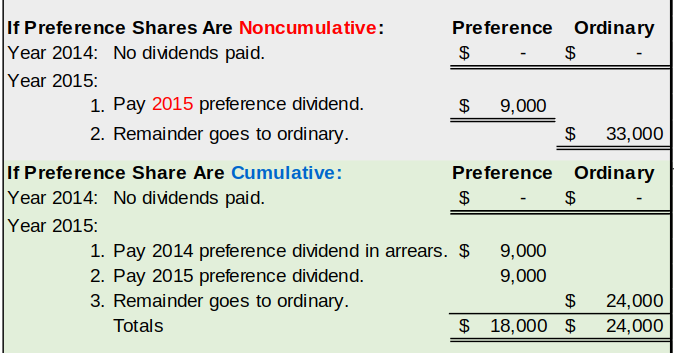
\includegraphics[width=1\columnwidth]{images/c9/preference_shares.png}
	\end{figure}
	
	
	\subsubsection{Treasury Shares}
	
	Corporations often buy their own shares back in the market. Repurchased 
	shares are called treasury shares. They do this because:
	\begin{itemize}[noitemsep]
		\item They want to send a signal that they believe the shares are worth 
		acquiring.
		\item Increase their shares needed to use in the acquisition of 
		another company.
		\item Increase shares for use in employee share option plans. 
		\textbf{Share options} will allow employees to purchase the shares of 
		the company’s share at a later date at a fraction of the share’s market 
		price.
		\item Reduce the number of outstanding shares to increase per-share 
		measures of earnings.
	\end{itemize}
	
	Cash dividends are not paid on treasury stock, and a corporation holding 
	its own shares cannot vote using these shares at the annual meeting. 
	Treasury share is not an asset. It is reported in the Shareholders’ Equity 
	portion of the balance sheet as a reduction from total equity. Treasury 
	share is usually recorded at the cost to purchase it, and the total cost of 
	all shares of treasury stock held by the company is the amount reported as 
	a reduction in Stockholders’ Equity.
	
	\begin{figure}[ht]
		\centering
		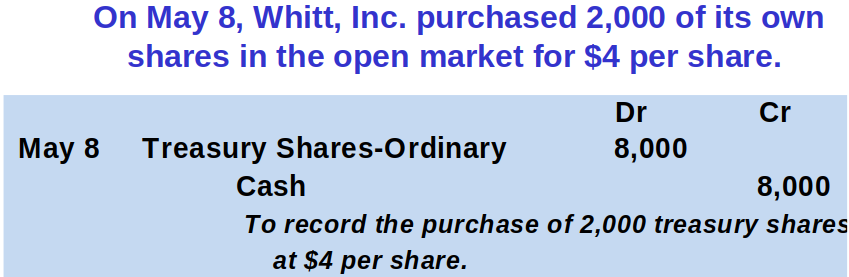
\includegraphics[width=1\columnwidth]{images/c9/purchase_treasury.png}
		\caption{Buying Treasury Shares}
		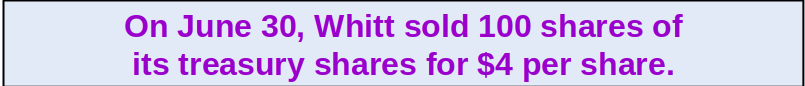
\includegraphics[width=1\columnwidth]{images/c9/selling_treasury.png}
		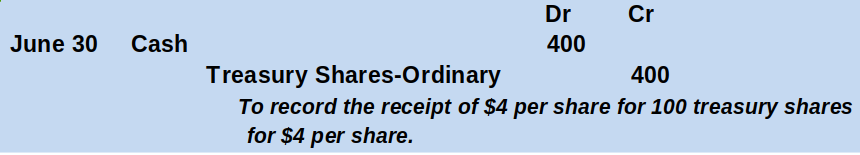
\includegraphics[width=1\columnwidth]{images/c9/selling_treasury_2.png}
		\caption{Selling Treasury Shares at Cost}
		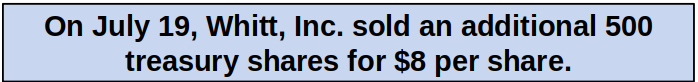
\includegraphics[width=1\columnwidth]{images/c9/sell_treasury_above.png}
		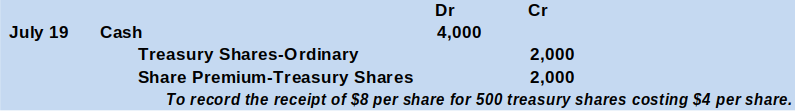
\includegraphics[width=1\columnwidth]{images/c9/sell_treasury_above2.png}
		\caption{Selling Treasury Shares Above Cost}
		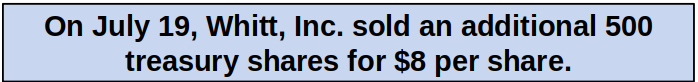
\includegraphics[width=1\columnwidth]{images/c9/sell_treasury_above.png}
		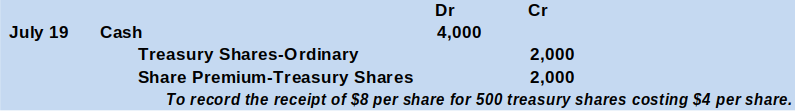
\includegraphics[width=1\columnwidth]{images/c9/sell_treasury_above2.png}
		\caption{Selling Treasury Shares Above Cost}
		
\includegraphics[width=1\columnwidth]{images/c9/treasury_below.png}
		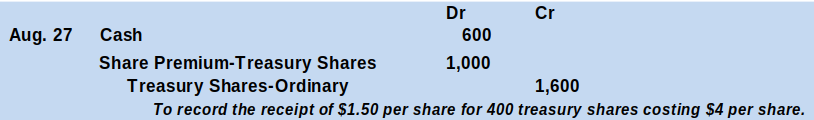
\includegraphics[width=1\columnwidth]{images/c9/treasury_below2.png}
		\caption{Selling Treasury Shares Below Cost}
	\end{figure}

	When the credit balance in this premium account is eliminated, any 
	remaining difference between the cost and selling price is debited to 
	Retained Earnings.
	
	A company never reports a loss (or gain) from the sale of treasury shares. 
	Note that in all the sale transactions, we credit the account Treasury 
	Shares at cost.
	
	\subsection{Statement of Profit or Loss and Other Comprehensive Income}
	
	The corporation must present a statement of profit or loss and other 
	comprehensive income which is intended to show  all non-owner changes in 
	equity and other comprehensive income. The statement of profit or loss and 
	other comprehensive income can be shown as a single statement. 
	
	\begin{figure}[ht]
		\centering
		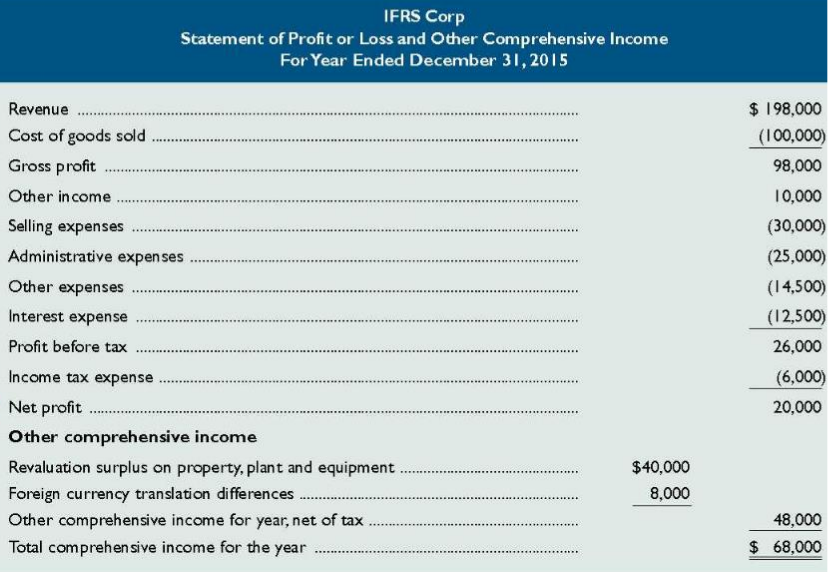
\includegraphics[width=1\columnwidth]{images/c9/statement_comprehensive.png}
	\end{figure}
	
	Alternatively, the  statement of profit or loss and other comprehensive 
	income can be presented as two statements: 
	\begin{itemize}[noitemsep]
		\item An income statement which 
		presents revenues and expenses recognized in the calculation of profit 
		or loss, and
		\item a statement of profit or loss and other comprehensive income 
		which begins with the profit or loss from the income statement and then 
		lists other items of income and expense \eg revaluation gains to 
		show total  comprehensive income.
	\end{itemize}
	
	\subsection{Statement of Changes in Equity}
	
	The  corporation  must  present  a  statement  of  changes  in  equity,  
	which  is  intended  to  show  all  owner changes in equity and dividends. 
	This statement includes the total amount of comprehensive income but its 
	main purpose is to show the amounts of transactions with shareholders 
	\eg  share issues and dividends, and to provide a reconciliation of the 
	opening and closing balance of each class of equity and each reserve. The 
	statement of changes in equity also shows the effects of any changes in 
	accounting policies and correction of prior period errors.
	
	\begin{figure}[ht]
		\centering
		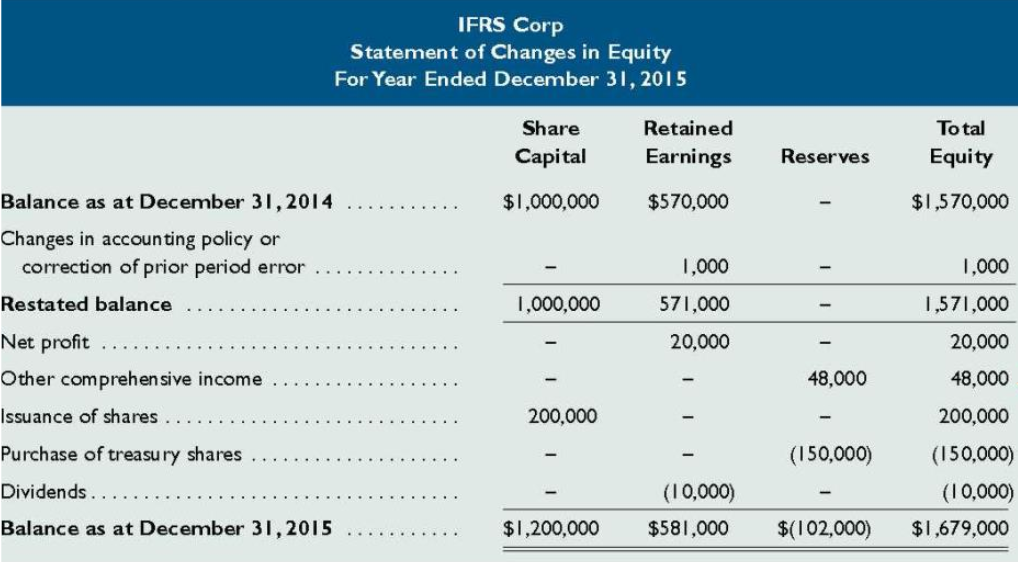
\includegraphics[width=1\columnwidth]{images/c9/sce.png}
	\end{figure}
	
	\subsection{Reserves}
	
	Most reserves result from accounting standards to reflect certain 
	measurement changes in equity rather than the income statement: for 
	example, asset revaluation surplus, foreign currency translation reserve, 
	and other statutory reserves. Retained earnings are also called 
	\textbf{revenue reserves}. A company's cumulative net profit less any net 
	losses and dividends declared dividends its inception.
	
	
	
	
	
	
	
	
	
\end{document}